\documentclass[10pt]{article}
\usepackage[polish]{babel}
\usepackage[utf8]{inputenc}
\usepackage[T1]{fontenc}
\usepackage{amsmath}
\usepackage{amsfonts}
\usepackage{amssymb}
\usepackage[version=4]{mhchem}
\usepackage{stmaryrd}
\usepackage{graphicx}
\usepackage[export]{adjustbox}
\graphicspath{ {./images/} }

\title{GIMNAZJUM }

\author{}
\date{}


\newcommand\Varangle{\mathop{{<\!\!\!\!\!\text{\small)}}\:}\nolimits}

\begin{document}
\maketitle
\begin{enumerate}
  \item Wiedząc, że czworokąt \(A B C D\) jest równoległobokiem, \(A E=B E=E D\) oraz że \(\Varangle A E D=78^{\circ}\), wyznacz miarę kąta \(B D C\).\\
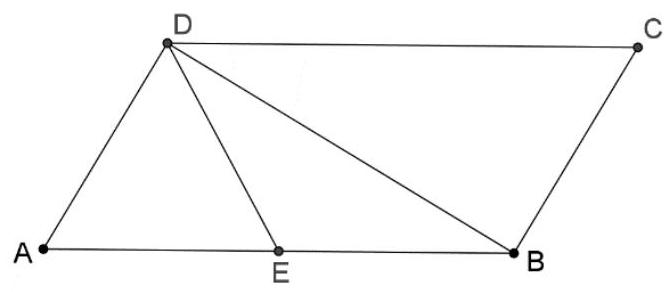
\includegraphics[max width=\textwidth, center]{2024_11_21_832da7521aa701459acfg-1(1)}
  \item Dany jest trójkąt \(A B C,|A C| \neq|B C|\). Wykaż, że symetralna boku \(A B\) i dwusieczna kąta \(A C B\) przecinają się na okręgu opisanym na trójkącie \(A B C\).
  \item Punkt O jest środkiem okręgu opisanego na trójkącie ABC. Punkt \(D\) jest rzutem prostokątnym punktu \(C\) na prostą \(A B\). Wykazać, że \(\Varangle A C D=\Varangle B C O\).\\
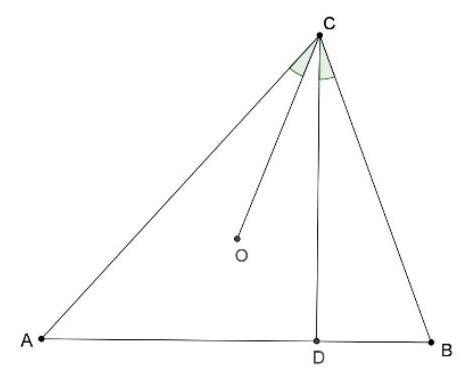
\includegraphics[max width=\textwidth, center]{2024_11_21_832da7521aa701459acfg-1(2)}
\end{enumerate}

\section*{LICEUM}
\begin{enumerate}
  \item Wiedząc, że \(A D=D B, A C \perp B C\) oraz, że \(\Varangle C E F=35^{\circ}\) i \(\Varangle A B C=28^{\circ}\), wyznacz miarę kąta EGD.
  \item Dany jest trójkąt \(A B C\). Niech \(K, L, M\) będą środkami łuków \(B C, C A\) i \(A B\) (nie zawierających wierzchołków trójkąta) okręgu opisanego na \(A B C\). Wykazać, że punkt\\
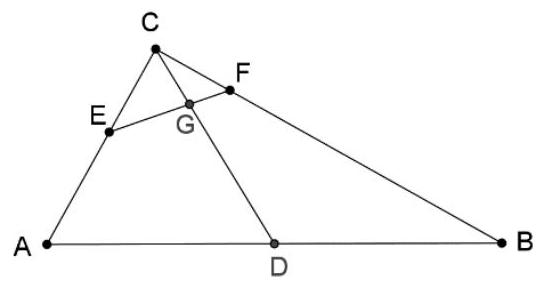
\includegraphics[max width=\textwidth, center]{2024_11_21_832da7521aa701459acfg-1}\\
przecięcia wysokości trójkąta \(K L M\) i środek okręgu wpisanego w trójkąt \(A B C\) pokrywają się.
  \item Dany jest trójkąt ostrokątny \(A B C\), przy czym \(\Varangle A C B=60^{\circ}\). Punkty \(D\) i \(E\) są rzutami prostokątnymi odpowiednio punktów \(A\) i \(B\) na proste \(B C\) i \(A C\). Punkt \(M\) jest środkiem boku \(A B\). Wykazać, ze trójkąt \(D E M\) jest równoboczny.
\end{enumerate}

\end{document}